%---=---==---===---====---=====---======---=====---====---===---==---=---%
%-                                DESIGN                                -%
%---=---==---===---====---=====---======---=====---====---===---==---=---%

\chapter{Design}\label{chap:design}

With the requirements formalised, the next stage is to propose potential designs which aim to solve the problems described in \cref{sec:challenges} by meeting the problem-specific requirements (\cref{chap:requirements}). This chapter will first touch on the methods used for design capture, then move into the system design and architecture, ensuring to discuss the strengths and weaknesses of each aspect of the design, and will finish with choosing a set of design proposals for implementation.

\section{Capture}

Several methods for capturing software design exist, with each having merits and pitfalls. This section aims to detail the four main methods used for design capture in this project: white-boarding, brainstorming, and wire-framing. Each technique will be concisely described, and reasons will be given as to why they were used.

\subsubsection{White-boarding}
Prototyping is a method used for design capture, which is akin to the first draft of a design. A whiteboard was chosen for this project due to its large canvas, and ease of addition and removal of ideas, though other materials are also for prototyping, such as pen and paper. Prototyping is worthwhile because it acts fast, allowing ideas to be drawn out immediately upon conception, however, its downsides are that it is informal as the ideas are only rough sketches and end up looking vastly different to the final design. Examples of this technique can be found in \cref{fig:architecture,fig:handdrawngui}.

\subsubsection{Brainstorming}
Another method for design capture is brainstorming; this is where a group of people communicate together to validate and combine their ideas. Brainstorming is beneficial to the design process because it involves multiple participants, preferably from diverse backgrounds and harbouring different viewpoints, which means that the ideas spawned will be more varied than when done individually. On the other hand, brainstorming can be ineffective if the conversation is not kept on topic, which can be difficult to do without relevant experience. Also, ideas can be sub-par, especially if the sample group is not well chosen. The instance of brainstorming in this project can be found in \cref{fig:brainstorm}.

\subsubsection{Wire-framing}
Additionally, wireframing is more formal than prototyping and serves as a final design that will be used in the implementation. A good aspect of wireframing is that it requires little training, meaning that the designs are undergone almost straight away. It also provides a more accurate representation of the final product, unlike the prototyping method described above, instances of these methods are compared in \cref{fig:gui}.

\section{Architecture}

To begin with, an overall system architecture design must be established to satisfy \cref{req:selfcontained}; this will be done before delving into the high-level design choices of each stage because it outlines a clear path for the project, sharpens focus, and provides specific goals to work towards. This section will expand on the stages of the white-boarded solution found in \cref{fig:architecture}.

\begin{figure}
    \centering
    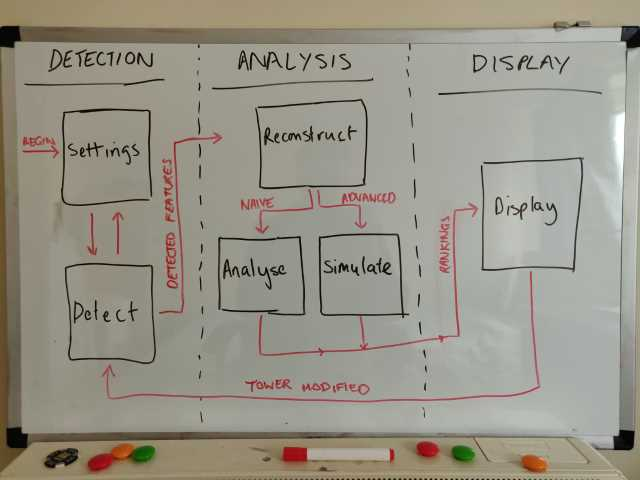
\includegraphics[width=0.6\linewidth]{images/design/architecture}
    \caption{System Architecture}
    \label{fig:architecture}
\end{figure}

\subsubsection{Settings}

When entering the system (top left of \cref{fig:architecture}) the user must begin with configuring settings for the application. These settings include items such as the number of blocks to detect, which analysis method to use, and how to display the results.

\subsubsection{Detection}

After the user has configured settings, the flow of the application should move into the detection stage. Here the user can use their camera, likely on the back of their phone, to scan and detect the blocks. The method used to detect the blocks will be marker based, which means that the user needs to move around the tower with their camera to detect each block individually, the benefits of using this method are described later in \cref{sec:des:detection}. During the detection, the user should be able to move back into the settings screen, in the case that their settings are causing the blocks to be inaccurately detected, or move onto the analysis stage.

\subsubsection{Reconstruction}

The analysis stage, shown in the centre of the figure separated from other stages with vertical dotted lines, is accessed from the detection stage by passing detection data, indicated by a red, arrowed line labelled \textit{Detected Features}.  Without delay (\cref{req:realtime}), the system should use these data to reconstruct the real world tower in three-dimensional virtual space; this could be done by instantiating block objects between markers on end faces of each block,  which is a parts-based modelling approach. Two arrows then emerge from the reconstruction section, moving into the naive or the advanced analysis method respectively.

\subsubsection{Heuristics}
If the user has chosen to use the \textit{naive} analysis approach, then the system will use a set of rules to determine the block removal feasibilities (\cref{req:rank}), and this includes rules such as the following that will be expanded upon later:
\begin{itemize}
    \item Set any blocks which singularly occupy their layer to have a low removal feasibility
    \item Set any central blocks which are neighbouring two side blocks to have a high removal feasibility
\end{itemize}

\subsubsection{Simulation}

Alternatively, the system will move into the simulation section in which the virtual tower is subject to numerous physics simulations to more accurately predict block removal feasibility. An example of the simulations used is to remove a block, then waiting a specified amount of time to test whether or not the tower remains stable, followed by resetting the tower state and iterating through the remaining blocks, resulting in a stability score for each block.

\subsubsection{Visualisation}

To end with, the \textit{Rankings} arrow shows movement between the analysis and display stages. Rankings, otherwise referred to as block removal feasibility rankings, are received and displayed in the format chosen by the user earlier, in the settings screen. Methods for display should include augmented reality (\cref{req:augment}), and can include \jenga{} variations (\cref{req:variants}), such as challenges, handicaps, and a points system.

The display stage should also allow the user to enter back into the detection stage (see \textit{tower modified} arrow at the bottom of \cref{fig:architecture}) because the real-world tower will eventually be modified by the user, rendering the current analysis useless, so the system state will need recalculating.

\section{\detection}\label{sec:des:detection}

Now that an overall architecture has been proposed, the method for the marker-based detection must be refined. Please refer to \cref{sec:markerless} for analysis into why marker-based was chosen over markerless detection, and \cref{code:houghpy} for the short program written to validate a markerless detection method. It has already been established (\cref{subsec:detectionsummary}) that UcoSLAM is the most appropriate method for the detection of blocks in a camera frame, but there is still a critical design choice that needs to be made, namely how exactly to affix markers to the blocks.

\subsection{Marker Affixation}\label{sec:markeraffixation}

\citet{arucopaper} explain that the smaller the marker, the more prone it is to errors during detection, however original \jenga{} blocks have faces that are just 15mmx25mm in dimensions, meaning that a margin of error cannot be avoided. To minimise the potential for errors, the markers must be as large as possible on the face, without being so large as to confuse the detection algorithm between multiple close-by markers.

\cref{fig:markersonblocks} shows one way to affix markers to blocks in this project, in which square, double-sided, sticky pads were used. This solution is advantageous because sticky pads and paper-printed markers are cheap to acquire, and simple to apply. However, the operation of attaching 108 pads and markers is a tedious task, which means that it has low commercial viability as users are unlikely to want to attach markers to their blocks in this way. Despite this, the markers were detectable using the ArUco test executable, as shown in \cref{fig:markersonblockswithposes}, in which the three axes and a box are drawn around the detected markers.

\begin{figure}[ht]
\centering
\begin{minipage}{0.45\textwidth}
  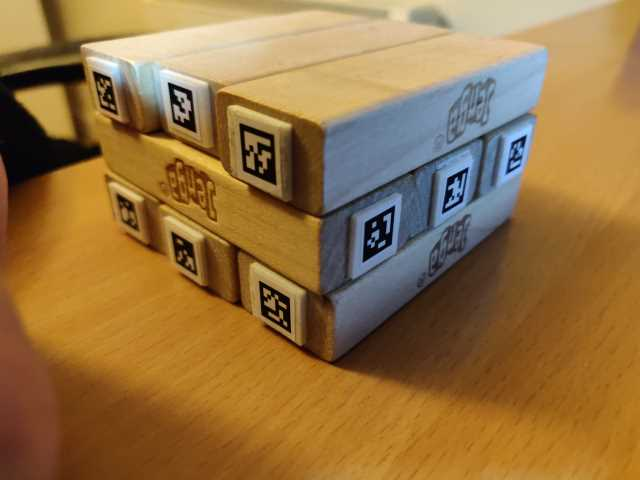
\includegraphics[width=\linewidth]{images/design/markersonblocks}
  \caption{Markers stuck to blocks}
  \label{fig:markersonblocks}
\end{minipage}
\begin{minipage}{0.45\textwidth}
  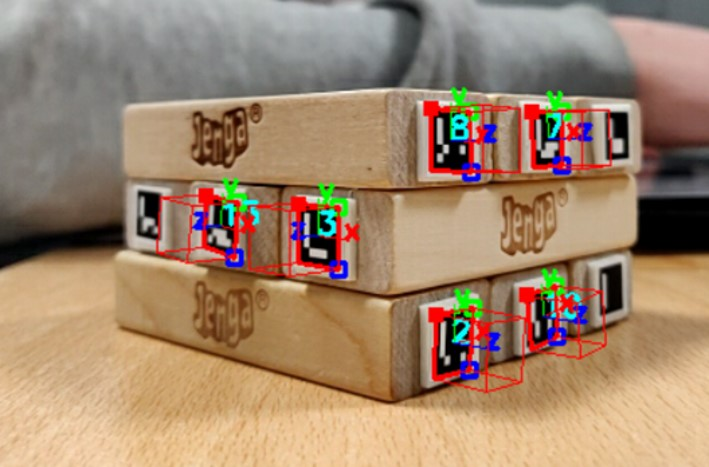
\includegraphics[width=\linewidth]{images/design/markersonblockswithposes}
  \caption{Detected poses and boxes}
  \label{fig:markersonblockswithposes}
\end{minipage}
\end{figure}

Another way to affix markers to blocks is by using a laser cutter. To do this, the blocks can either be cut individually, all together at once, or at some point in between the two. The benefit of cutting the blocks individually is that it is easier to centre the block under the laser to ensure the marker is cut in the middle, which increases the minimum distance between markers on separate blocks, yet this method is just as monotonous as using sticky pads. Also, any blocks which have misaligned marker placement could be thrown out at the loss of just one block each time.

Conversely, cutting all the blocks at once allows for significantly less cutting time, but brings about the risk of misalignment on multiple blocks at a time, coincidentally this did happen and can be seen in \cref{fig:misalignment}. The slight variations in block sizes, multiplied by the number of blocks bound together, meant that rows of the bound blocks were misaligned, hence the laser cut in the wrong places. In addition to this problem, the laser cutter used did not have any in-built alignment tools, so blocks had to be positioned by hand, leading to human error.

\begin{figure}[ht]
\centering
\begin{minipage}{0.45\textwidth}
  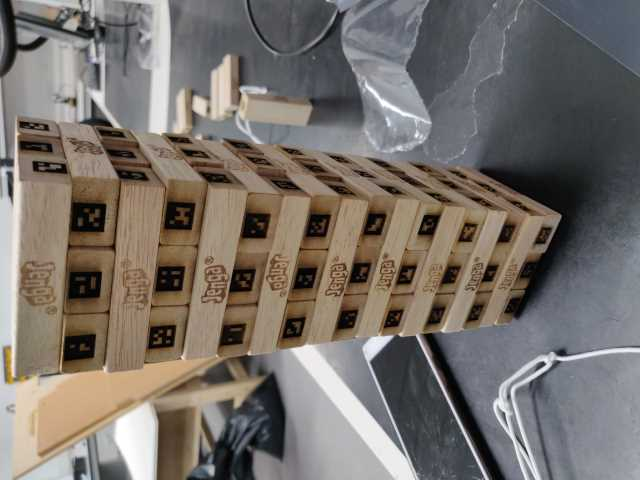
\includegraphics[width=\linewidth]{images/design/misalignment}
  \caption{Misalignment during the cutting process}
  \label{fig:misalignment}
\end{minipage}
\begin{minipage}{0.45\textwidth}
  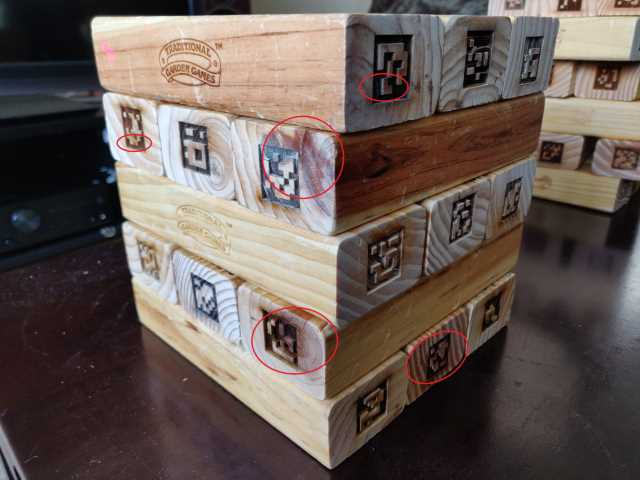
\includegraphics[width=\linewidth]{images/design/largeblocks}
  \caption{Large blocks with markers, red circles indicate colour variation}
  \label{fig:largeblocks}
\end{minipage}
\end{figure}

After several attempts and various methods of aligning blocks in the laser cutter it was decided that such a task was too difficult to accomplish to the degree of precision needed. A solution to this was to use blocks of greater size, this is because the faces of the larger blocks could allow for relatively smaller markers, thus reducing the risk of misalignment. Still, there were problems. The big blocks used had different wood grain and texture, leading to variations in colour and brightness, these are pointed out in \cref{fig:largeblocks}, and due to this, some blocks were unable to be detected by the ArUco library.

In summary, affixing markers to blocks is not as straightforward as it would seem and no method was found to have both ease of setup and low error rate. Despite this, the sticky pad and paper method should be adopted for the implementation because of its success in low error detection.

\section{\analysis}

Moving forward, the analysis stage must be addressed. Following \cref{req:rank}, this stage has to use the detected features data to reconstruct the tower in a virtual space, and then calculate rankings for block removal feasibility for later display. This section details design choices made for both \nameref{subsec:heuristics} and \nameref{subsec:simulation} analysis.

\subsection{Heuristics}\label{subsec:heuristics}

One way in which to approach the analysis problem is to use a set of simple rules to determine block removal feasibility rankings, these are described below, with reasons given as to why they were chosen. In the rule set, it is assumed that there are three blocks per layer, referred to as two side blocks, and one central block. Also, the red cross in the diagrams show which block is to be removed.

\begin{enumerate}
    
	\item \textbf{Constraint:} Any block which singularly occupies its layer.
	\\\textbf{Feasibility of removal:} Low.
	\\\textbf{Reason:} All above layers would fall by one block height, which adds risk if the tower is already unstable.
	
	 \begin{figure}[ht]
        \centering
        \begin{minipage}{.3\textwidth}
            \centering
            \drawblockrow{1}{}{}{1}
        \end{minipage}\hfill
        \begin{minipage}{.3\textwidth}
            \centering
            \drawblockrow{}{1}{}{2}
        \end{minipage}\hfill
        \begin{minipage}{.3\textwidth}
            \centering
            \drawblockrow{}{}{1}{3}
        \end{minipage}
        \caption{Possibilities for Rule 1}
    \end{figure}
	
	\item \textbf{Constraint:} Any side block which is situated on a layer with only one other side block.
	\\\textbf{Feasibility of removal:} Low.
	\\\textbf{Reason:} The above layers would pivot around the remaining side block, causing the tower to fall.
	
	\begin{figure}[ht]
	\centering
	\begin{minipage}{.45\textwidth}
        \centering
        \begin{minipage}{.45\textwidth}
            \centering
            \drawblockrow{1}{}{1}{1}
        \end{minipage}
        \begin{minipage}{.45\textwidth}
            \centering
            \drawblockrow{1}{}{1}{3}
        \end{minipage}
        \caption{Possibilities for Rule 2}
    \end{minipage}
    \begin{minipage}{.45\textwidth}
        \centering
        \begin{minipage}{.45\textwidth}
            \centering
            \drawblockrow{1}{1}{}{1}
        \end{minipage}
        \begin{minipage}{.45\textwidth}
            \centering
            \drawblockrow{}{1}{1}{3}
        \end{minipage}
        \caption{Possibilities for Rule 3}
    \end{minipage}
    \end{figure}
	
	\item \textbf{Constraint:} Any side block which is situated on a layer with only one other central block.
	\\\textbf{Feasibility of removal:} Medium.
	\\\textbf{Reason:} The centre of mass of the above layers is usually near the middle of the tower, so this side block is unlikely to be bearing weight.
 	
 	\item \textbf{Constraint:} Any central block which is situated on a layer with only one other side block.
    \\\textbf{Feasibility of removal:} Low.
    \\\textbf{Reason:} The above layers would pivot around the remaining side block, causing the tower to fall.
	
	\begin{figure}[ht]
	\centering
	\begin{minipage}{.6\textwidth}
        \centering
        \begin{minipage}{.45\textwidth}
            \centering
            \drawblockrow{1}{1}{}{2}
        \end{minipage}
        \begin{minipage}{.45\textwidth}
            \centering
            \drawblockrow{}{1}{1}{2}
        \end{minipage}
        \caption{Possibilities for Rule 4}
    \end{minipage}
    \begin{minipage}{.3\textwidth}
        \centering
        \begin{minipage}{0.9\textwidth}
            \centering
            \drawblockrow{1}{1}{1}{2}
        \end{minipage}
        \caption{Rule 5}
    \end{minipage}
    \end{figure}
	
	\item \textbf{Constraint:} Any central block which neighbours two side blocks.
	\\\textbf{Feasibility of removal:} High.
	\\\textbf{Reason:} Neighbouring side blocks act as stabilisers.
	
	\item \textbf{Constraint:} Any side block situated on a full layer.
	\\\textbf{Feasibility of removal:} Medium.
	\\\textbf{Reason:} The centre of mass of the above layers is usually near the middle of the tower, so this side block is unlikely to be bearing weight.
	
	\begin{figure}[ht]
        \centering
        \begin{minipage}{.3\textwidth}
            \centering
            \drawblockrow{1}{1}{1}{1}
        \end{minipage}
        \begin{minipage}{.3\textwidth}
            \centering
            \drawblockrow{1}{1}{1}{3}
        \end{minipage}
        \caption{Possibilities for Rule 6}
    \end{figure}
	
\end{enumerate}

This method is good because it is simple to implement, and also has low complexity and runtime. However, it assumes the blocks will be aligned with the tower in the same way that they were in the starting state, yet it is likely that the blocks will rotate and translate from their original positions as the game progresses, meaning that this analysis would lose truth with changes to the tower state, thus providing a poor estimate for ranking.



\subsection{Simulation}\label{subsec:simulation}

A more advanced method for analysis would be to use physics simulation software, which allows developers to implement the laws of physics into their applications. Simulation software could be used to determine more accurate removal feasibility rankings than the \nameref{subsec:heuristics} method because it takes into account more advanced physics features, thus adding realism to the analysis. In this section, two physics simulators, Unity and Project Chrono, are compared, before the design for the simulation program is described.

\subsubsection{Software}

\cite{projectchrono} is an open-source physics engine specialised for use with robotics and biomechanics, but is capable of supporting much more. Advantages to using Chrono are that it is highly customisable, with realistic physics, and can be compiled to Android (\cref{req:android}). On the other hand, it has a steep learning curve and is not natively packaged with a GUI.

In contrast, \cite{unity} is primarily a game engine that runs on the PhysX engine. It also brings native support for Android, but does come with a built-in GUI that has drag and drop functionality and is easy to get started with. In addition, Unity has a large community with lots of support and wikis, which means that there will be people to whom to turn if problems are encountered. It is because of these benefits over Chrono that it was decided to use Unity for the simulation software.

\subsubsection{Simulation Design}

After deciding to use Unity as the software for simulation, the next step is to decide what will take place in the simulations, and how to score the removal feasibility rankings for each block.

The first, and simplest way to do this is to build the tower from the block poses, then systematically remove each block and calculate whether or not its removal causes the tower to fall over. To calculate is the tower is left standing, the simulation could wait a specific amount time, and then check if the highest block is still at the same level that it was before block removal. This method gives a good indication of the vitality of each block with regard to tower stability, however, it only produces binary output; \textit{fallen} or \textit{standing}, and it could also give a \textit{fallen} result if a whole row is removed at once, which is a legal move in the game. Furthermore, it does not consider the movement of the removal block, as it will just be destroyed in position, which means that it ignores real-world factors such as rotation and friction.

The above method can be improved by giving a more distributed score for the set of blocks. This could be done by either calculating the time it takes for the tower to fall, and using that value to scale the results. Another way involves waiting a fixed amount of time after removal, and then finding out how far the furthest block has travelled from the centre of the tower. Both of these techniques would produce a similar outcome, and so they should be tested in the \nameandsecref{chap:implementation}.

Moreover, it could also be improved by changing the way blocks are removed from the tower. Instead of destroying each block in place, the simulation could attempt to pull the block out from the tower. There are a few constraints on how it is possible to remove blocks from a tower while trying to minimalise disturbance \citep{jengaanalysis}; central blocks can only be moved perpendicularly to the tower, whereas side blocks can be removed by rotation or translation away from the tower. This may prove difficult to simulate because the previous work done in this area showed that finding the correct physics properties for realistic block removal is no easy task, nonetheless, effort should be made to implement this later on, as removing the blocks in this way provides a more accurate representation of how they would be removed in the real world.

\begin{figure}
    \centering
    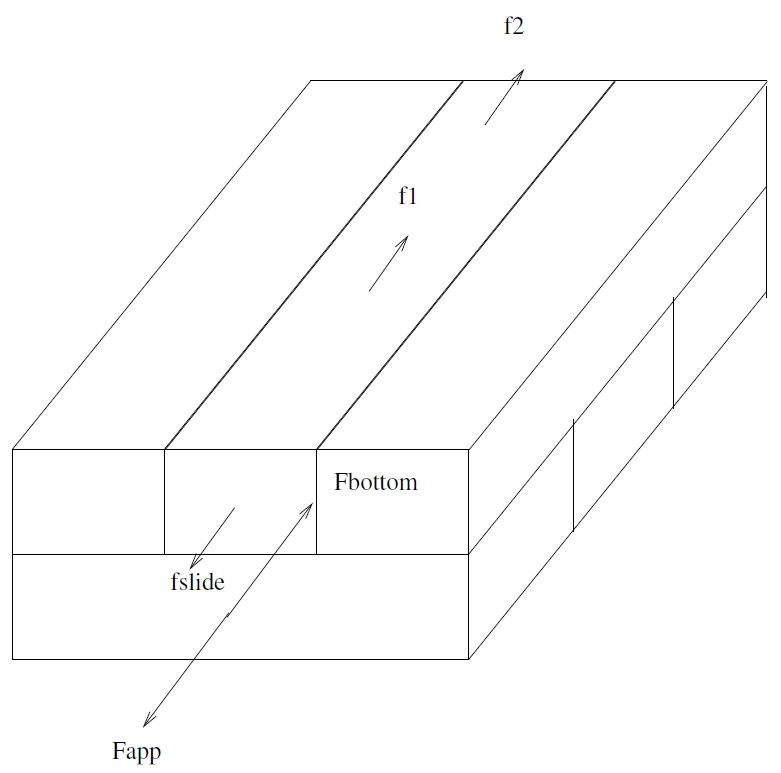
\includegraphics[width=.4\textwidth]{images/design/analysisjengamovement}
    \caption{Central block removal, image from \citet{jengaanalysis}}
    \label{fig:centralblockremoval}
\end{figure}

\section{\display}

Designing the visualisation stage is subsequent to finalising designs for detection and analysis. This section aims to cover both what to display (\cref{subsec:variation}) and how to display (\cref{subsec:tools}) the removal feasibility rankings to the user.

\subsection{Tools}\label{subsec:tools}

There are various tools and kits available for augmented reality display, of which, ARCore and OpenCV are two of the most prominent at this time. Solutions using these software are described below.

\subsubsection{ARCore}

ARCore is an augmented reality software development kit built for Android smartphones, similar to ARKit for iOS smartphones, that can be paired with other software such as Unity for extensibility. One solution using ARCore includes using the virtual tower built earlier in Unity, and displaying that on the phone screen. With ARCore it is possible to track the environment and place virtual objects directly onto planes, the solution should make use of this feature by allowing the user to generate the virtual tower on the same plane that the real tower is occupying. Having the two towers side by side means that the user can compare them efficiently, which satisfies \cref{req:stageunderstand} for ease of use.

\begin{figure}[ht]
\begin{minipage}{\textwidth}
    \centering
    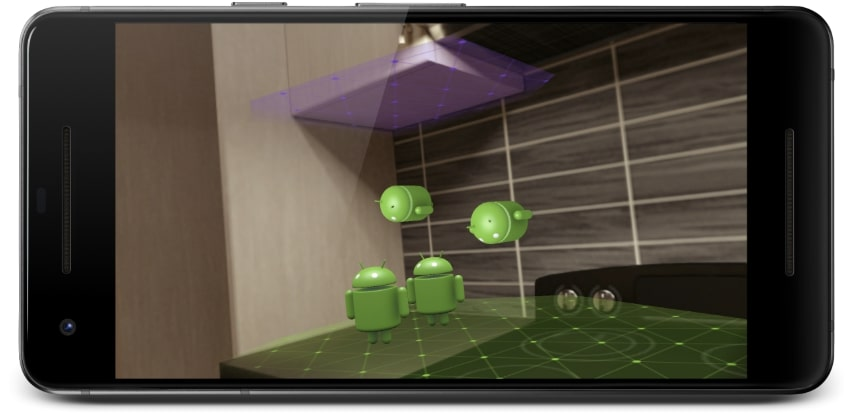
\includegraphics[width=.8\textwidth]{images/design/andyandroid}
    \caption{An example of using ARCore to place virtual objects onto a real plane, image from this  \protect\footurl{https://developers.google.com/ar/develop/unity/quickstart-android}{ARCore Sample}}
    \label{fig:andyandroid}
\end{minipage}
\end{figure}

Another way to display the tower with ARCore is to place the virtual tower directly on top of the real tower so that only the virtual tower is visible. Doing this provides a more immersive experience to the user, which means that they are less likely to lose attention (\cref{req:attention}). However, ARCore does not allow for tracking of multiple individual objects, so when the user tries to take a block from the tower, only the physical piece will be removed, leaving the virtual in its place; this may be unexpected behaviour to the user and could result in confusion, which is detrimental to the success of the system.

\subsubsection{OpenCV}

Alternatively, OpenCV could be used for the display. While the previously mentioned method pairs well with Unity, this software goes hand in hand with augmented reality markers, which are already affixed to the blocks. The advantage of this method is that it can track the individual markers, meaning that the experience does not have to end when a block gets removed; it provides dynamic augmentation even during the process of removal, unlike the ARCore method.

\subsubsection{Virtual}

On the other hand, a solution exists without the use of AR, that is to present the information in virtual reality. Again, this method uses Unity, but instead of placing the virtual tower into the real environment, it stays on screen, with the ability to zoom in on different areas of the tower, and rotate to see other sides. However, when compared with the methods as mentioned earlier, this is less immersive and requires more work for the user; therefore it should not be used in the implementation.

\subsubsection{}
In summary, OpenCV should be the method of choice for displaying the results because it tracks the individual blocks at all times, contrary to the ARCore method. Yet, it would still be worthwhile to incorporate ARCore into the system as an extension, if time allows for it at the end of the project.

\subsection{Variation}\label{subsec:variation}
In this project, it would be adequate to take the raw block removal feasibility rankings and augment those numbers onto each block. While this would serve the purpose of the system, it may be beneficial to implement additional variations for reasons of aesthetics and increased gamification.

The method used to capture design solutions for these variations was brainstorming. Various ethics were considered before participants were engaged in this study, details of which can are in \cref{chap:ethics}. This section explains what each leaf of the mind-map in \cref{fig:brainstorm} represents:

\begin{figure}[ht]
  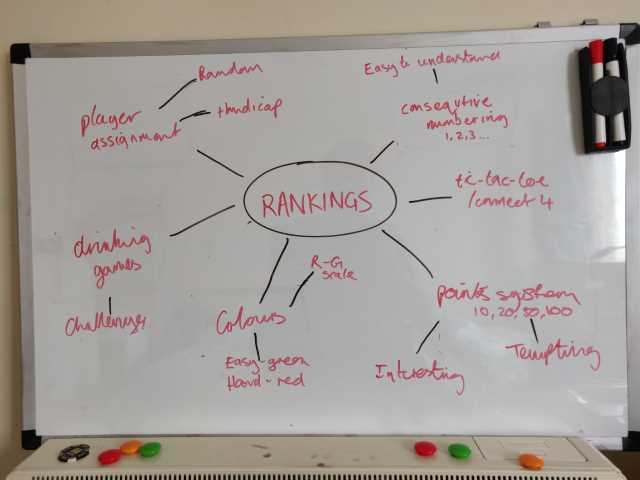
\includegraphics[width=\linewidth]{images/design/rankings}
  \caption{Brainstorm of game variants}
  \label{fig:brainstorm}
\end{figure}

\subsubsection{Consecutive Numbering}
The first variation considered was also the most blatant: consecutive numbering. In short, this means that the ranking should be displayed as is, beginning from 1, meaning most feasible to remove, and traversing through all the blocks to the least feasible, adding one to the counter at each block. This method is arguably the easiest to understand, and gives the user clear indication of the block ranks, although it lacks visuals, and therefore it would be less interesting than competing methods.

\subsubsection{Points System}
Extending from the consecutive numbering method is the points system; it differs from the numbering method as blocks are assigned ranks in bands. For instance, high feasibility blocks are designated to have 10 points, medium feasibility have 20 points, and low have 50 points. When a user removes a block, they receive the number of points that the block is worth, intending to end the game with the most points out of all players. This method is well-suited to \jenga{} because it adds an extra variable in consideration of which block to choose, making the game more interesting. Also, a 100 point band could be used for blocks which are deemed improbable to remove, tempting the more risk-averse players in for more points.

\subsubsection{Colours}
Maybe the most visual of the variants that evolved from the brainstorm is the colour variant, in which blocks are coloured based on their rank. Two ways this could be completed are by using a colour scale, or colour bands. The colour scale is a smooth transition from red to green, indicating the hardest and easiest blocks to remove respectively, which would be useful to the user as colours are good visual cues. On the other hand, colour bands could be used, for instance, red for difficult blocks, yellow for medium blocks, and green for easy blocks. Out of the two methods, the colour scale is preferred because it gives more information to the user.

\subsubsection{Tic-Tac-Toe / Connect 4}
An interesting suggestion was to incorporate minigames, such as tic-tac-toe and connect 4. Players work in teams to either pull out a certain number of blocks in a row, which would be 3 in the case of tic-tac-toe, or 4 in the case of connect 4. The visualisation for these variations is opposite to the ones already mentioned because they require the empty gaps to be augmented, which is more difficult to implement because the system does not implicitly know where gaps are in the tower.

\subsubsection{Player Assignment}
Moving to the left of \cref{fig:brainstorm}, is player assignment, this is where blocks are assigned to specific players at the start of the game, and players are restricted to only remove blocks assigned to them. Extending on this idea, the player assignments can be dynamic throughout the game, changing to give the harder blocks to the top players, as a handicap feature. This variant is worth considering because it makes the game more personal, which means that players are more likely to feel included.

\subsubsection{Challenges}
Finally, a drinking variant was proposed. After this suggestion, the study participant was advised that variants should be targeted towards all audiences, not just a specific group, such as those who drink alcohol; resulting from this, the variant was named \textit{Challenges} instead. The challenges variant involves assigning various tasks to each block at the start of the game, such as doing a star jump, or naming 5 capital cities. What is good about this variant is that the set of challenges are endless, and could even be set by the users, meaning that they can choose appropriate tasks for their player group.

\subsubsection{Summary}\label{sec:variantssummary}
The brainstorming activity was a success because the participants came up with six unique variants that could all be implemented into the system, which is more than was hoped for. Moving forward, the colour variant should be the first to be adopted, due to its pleasing aesthetics (\cref{req:aesthetics}), but other variants should not be forgotten about, and could be worked towards as an extension to the project.

\section{System}

The final section in this design chapter involves the overall system design and interface. It begins will an 

\subsection{Standalone}\label{sec:standalone}

Initially, a solution was white-boarded to achieve a quick and simple design, shown in \cref{fig:handdrawngui}. The Settings screen (left) contains only a few items; an input box for the number of blocks, a dropdown box to select the marker dictionary, and a button to move onto the Camera screen. An effort was made here to keep the design both simple and minimal, because too much information leads to poor design. Furthermore, the Camera screen (right) contains but two items, a full screen camera and a button to return to the Settings, these were chosen to aid in the immersion of the application.

\begin{figure}[ht]
\begin{minipage}{0.45\textwidth}
    \centering
    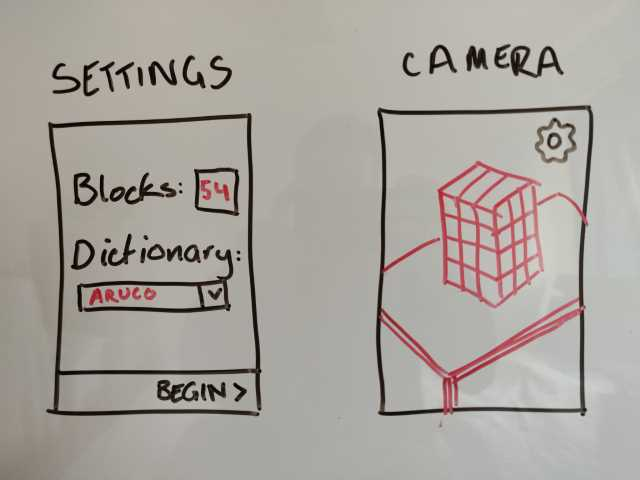
\includegraphics[width=0.9\textwidth]{images/design/gui}
    \caption{Hand-drawn}
    \label{fig:handdrawngui}
\end{minipage}\hfill
\begin{minipage}{0.45\textwidth}
    \centering
    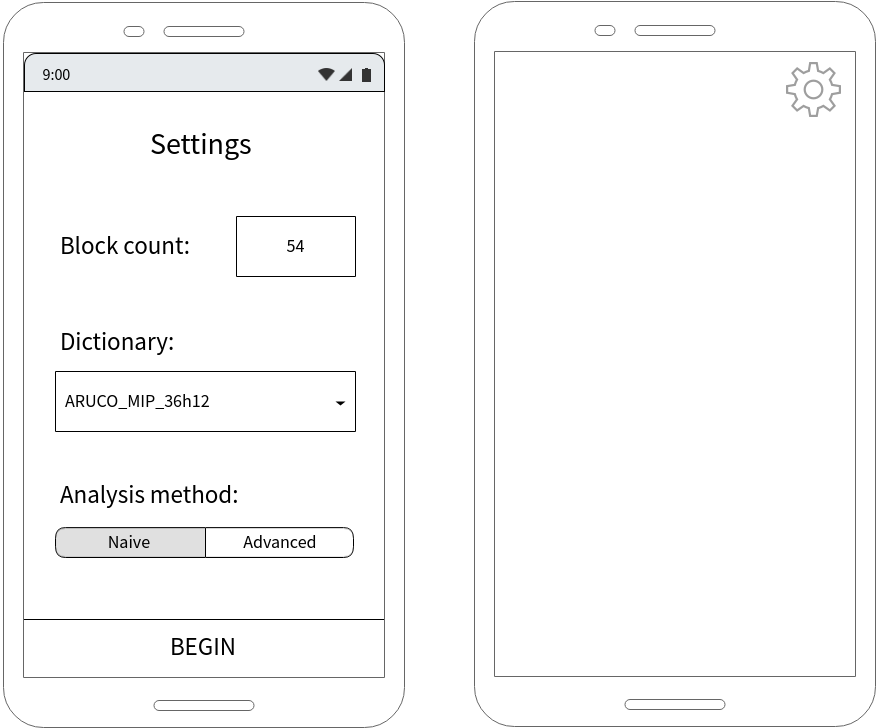
\includegraphics[width=0.9\textwidth]{images/design/wireframe}
    \caption{Wire-frame}
    \label{fig:wireframe}
\end{minipage}
\caption{Graphical User Interfaces}
\label{fig:gui}
\end{figure}

To formalise and improve the system design, a wire-frame model was created using the white-boarded solution as a template. Several changes were made to the settings, these were the addition of the analysis method, as well as a title, and centring the Begin button. With these changes, the design looks cleaner, and includes more of the desired functionality of the system. In contrast to the changes made to the Settings screen, there were no changes to the design of the Camera screen, this is because the design is minimal enough to include all the needed functionality, but not so little to cause confusion. For example, the Settings button could be removed in favour of a swipe action and to allow for a truly fullscreen camera, but some users would then find it difficult to navigate to the settings.

\subsection{Server / Client}

The documentation for \citet{ucoslam} states that one of the main features is:

\begin{displayquote}
\textit{``Multiplatform, ready to be compiled in Windows, Linux and Android systems''}
\end{displayquote}

However, several attempts to compile the library for Android failed. The approaches taken were widely varied, but including using different operating systems, i.e. Ubuntu 16, Ubuntu 18, and Windows 10, downgrading Android build tools, building older versions of OpenCV, compiling with legacy versions of the Android NDK, and various CMake option changes. On top of this, the developer of UcoSLAM was reached out to, but no response was received before the hand-in date. So, although the documentation claims to be ready to be compiled for Android systems, this was found not to be possible; thus a different system design had to be conceived.

The solution to the compilation problem in this paper is to switch from a standalone architecture to a client/server architecture, this is done in such a way that the client sends camera frames to the server which performs the localisation and mapping of markers, and then the server sends results back to the client. Developing the application in this way means that the software used to map markers is not restricted to running on a smartphone, which means that UcoSLAM can still be used in the project.

It is worth noting that changing to this architecture partially violates \cref{req:android} because part of the application now runs on a server, instead of an Android device, but there are significant advantages which outweigh this requirement violation. For instance, complexity has been removed from the Android app, meaning that it will be easier to maintain. Also, now there is an opportunity to move the analysis stage onto the server, which means that less compute heavy tasks need to run on the device, opening up the application to devices with slower hardware (\cref{req:lightweight}). With the analysis stage on the server, more complex simulations can be run, giving the potential for more accurate feasibility rankings, which improves on \cref{req:accuracy}.

\begin{figure}[ht]
    \centering
    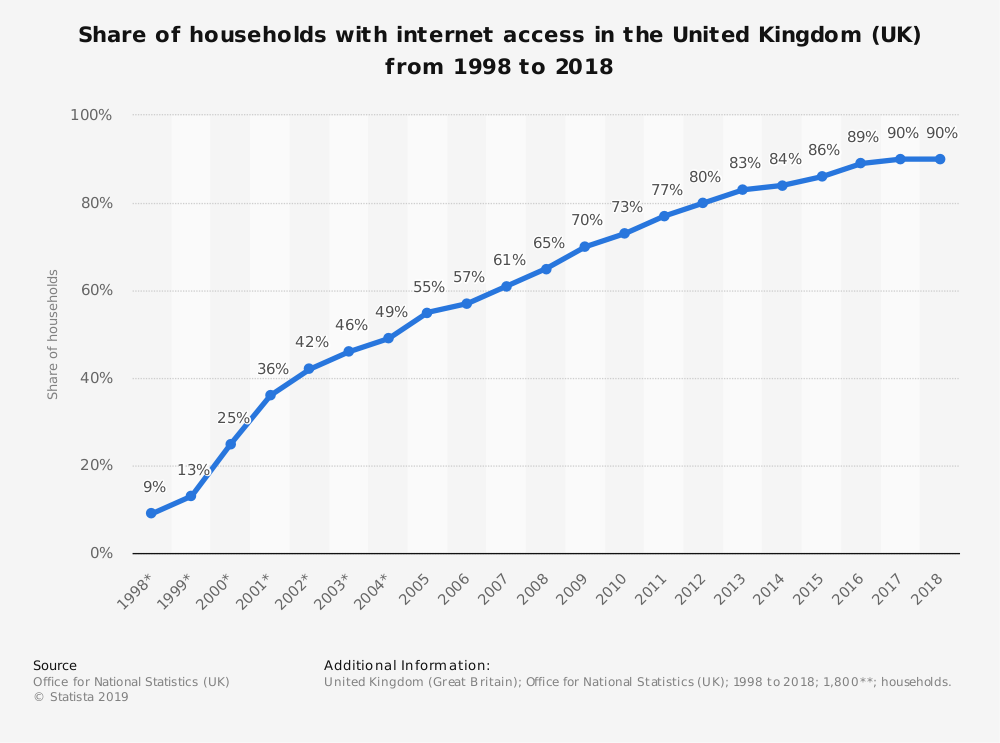
\includegraphics[width=.6\linewidth]{images/design/homeswithinternet}
    \caption{Households with internet access in the United Kingdom (UK), image from \cite{internetaccess}}
    \label{fig:internet}
\end{figure}

Disadvantages of the client/server approach include the need for a server to be present during the runtime of the application, this means that users are constrained to only using the app when they have a working internet connection, or can use a local server, such as a laptop or PC. However, today, this will generally not be an issue due to widespread internet access, for example, \cref{fig:internet} shows that 90\% of homes in the UK have access to the internet. Furthermore, adding a server into the system adds overall complexity, because inter-device communication has to be implemented.

\subsubsection{Changing Requirements}\label{subsec:changingrequirements}

Requirements were previously set under the assumption of a standalone system, but as a result in the change of architecture, new requirements were set and can be found in \cref{sec:req:additional}. One of the most crucial additional requirements (\cref{req:comms}) is that the communication with the server must be asynchronous, this means that a separate thread will be used to send and receive data, which is beneficial because the application will not be blocked from running when it decides to send a frame to the server. If the communication were blocking, then the camera activity in the app would seem jittery, as the screen would only update after completing send to the server, which can take an arbitrarily long time.

Another cause for concern, indicated by \cref{req:privacy}, is privacy. It is not unreasonable to assume that some images sent from the smartphone app will contain personal information, for example a postal item which contains the name and address of the user. For this reason, the server must not store any of the images it receives from a client, this is possible if frames are processed immediately and then thrown away when after pose information has been extracted.

\subsubsection{Design}

A high level overview of the responsibilities of the client and server is shown below in \cref{fig:clientserverarch}.

\begin{figure}[ht]
    \centering
    \begin{minipage}{.45\textwidth}
        \begin{tikzpicture}[grow cyclic, text width=2.7cm, align=flush center,
        	level 1/.style={level distance=3cm,sibling angle=72}]
         
        \node{Server}[clockwise from=160]
            child { node {Receive frames from client}}
            child { node {Identify block poses}}
            child { node {Reconstruct the tower}}
            child { node {Analyse block removal feasibility}}
        	child { node {Send ranks to client}};

        \end{tikzpicture}
    \end{minipage}\hfill
    \begin{minipage}{.45\textwidth}
        \begin{tikzpicture}[grow cyclic, text width=2.7cm, align=flush center,
        	level 1/.style={level distance=2.5cm,sibling angle=90}]
            \node{Client}[clockwise from=135]
            	child { node {Calibrate camera}}
            	child { node {Send frames to server}}
            	child { node {Receive ranks from server}}
            	child { node {Display}};
        \end{tikzpicture}
    \end{minipage}
\caption{High level responsibilities}
\label{fig:clientserverarch}
\end{figure}

\section{Summary}

This chapter has described and explained the design choices for the system. Next, this system will be implemented.